\section{Drittes Bonusfeature: Einstellungen der Tastenkürzel}\label{sec:keybindings-settings}
Die Tastenkürzel selbst festzulegen ist Bestandteil von vielen Spielen, daher wurde mit dem Kunden vereinbart, Einstellungen für die Tastenkürzel als drittes Bonusfeature zu entwickeln. Der Nutzer kann somit gewünschte Tasten für die Bewegung, Interaktion und das Öffnen des Pausemenüs festlegen. 
\subsection{Mockups}\label{subsec:mockups-keybindings-settings}
Das Einstellungsfenster für die Tastenkombinationen aus der Abbildung~\ref{fig: Einstellungen der Tastenkürzel} kann der Nutzer öffnen, indem er auf den Knopf 'Keybindings' in dem Einstellungsmenü aus der Abbildung~\ref{fig: Einstellungsmenü} drückt.
In der Abbildung~\ref{fig: Einstellungen der Tastenkürzel} sieht der Nutzer verschiedene Knöpfe, die einen Inhaltstext von der jetzig festgelegten Taste besitzen: vier Knöpfe für die Navigation, einen Knopf für die Interaktion und einen Knopf für das Öffnen des Pausemenüs. Darüber hinaus sind noch drei andere Knöpfe vorhanden, um jeweils zum Einstellungsmenü zurückzukehren, alle Tasten auf die voreingestellten Tastenkombinationen zurückzusetzen oder die Änderungen der Tastenkombinationen zu bestätigen.
\begin{figure}[H]
    \center
    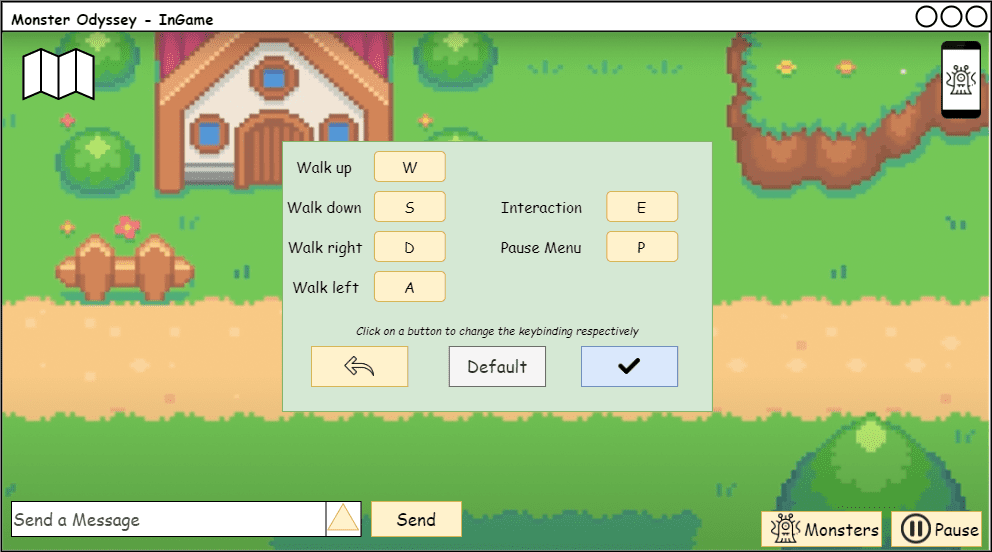
\includegraphics[scale=\scale]{images/mockups/Bonusfeatures/Keybindings/KeybindingsSettings.png}
    \caption{Mockup: Einstellungen der Tastenkürzel}
    \label{fig: Einstellungen der Tastenkürzel}
\end{figure}
\begin{figure}[H]
    \center
    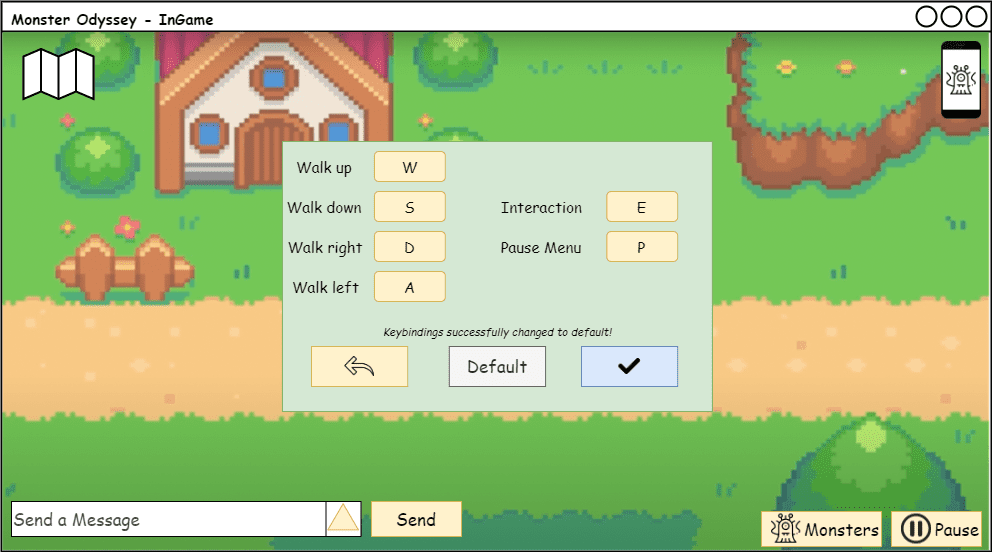
\includegraphics[scale=\scale]{images/mockups/Bonusfeatures/Keybindings/KeybindingsSettingsDefault.png}
    \caption{Mockup: Tastenkürzel zurückgesetzt}
    \label{fig: Tastenkürzel zurückgesetzt}
\end{figure}
Sobald der Nutzer beispielsweise einen Knopf der Navigationstasten drückt, wird der Inhaltstext dieser Taste mit „...“ wie in der Abbildung~\ref{fig: Knopf gedrückt} ersetzt und wird auf eine Eingabe vom Nutzer gewartet. Dabei wird der Nutzer zusätzlich in einem Text wie in Abbildung~\ref{fig: Knopf gedrückt} darauf hingewiesen, dass auf eine Eingabe gewartet wird. Der Inhaltstext wird mit der entsprechenden Taste, wie in Abbildung~\ref{fig: Tastenkürzel geändert} ersetzt, und ein Text für die Bestätigung angezeigt, wenn die Eingabe vom Nutzer erfolgt ist. Anschließend kann der Nutzer auf dem blauen Knopf aus der Abbildung~\ref{fig: Tastenkürzel geändert} drücken, um die Änderungen abzuschließen und zu speichern.
Möchte der Nutzer zu einem späteren Zeitpunkt mit den voreingestellten Tastenkombinationen weiterspielen, so kann er dies mit dem mittleren Knopf aus der Abbildung~\ref{fig: Einstellungen der Tastenkürzel} tuen. Es wird dabei die Aktion mit einem Text in demselben Fenster wie in der Abbildung~\ref{fig: Tastenkürzel zurückgesetzt} bestätigt.
\begin{figure}[H]
    \centering
    \begin{subfigure}[b]{0.4\textwidth}
        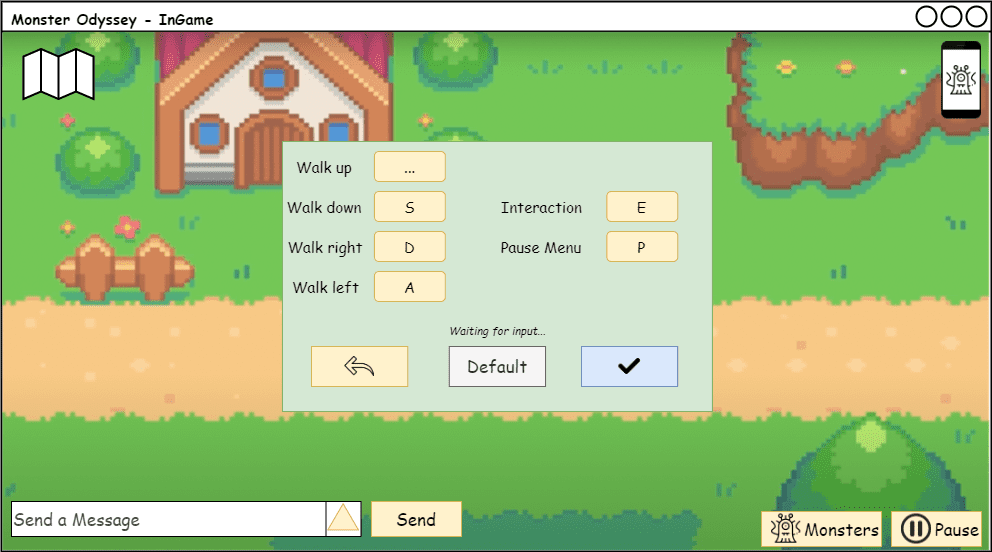
\includegraphics[width=\textwidth]{images/mockups/Bonusfeatures/Keybindings/KeybindingsSettingsWaitingForInput.png}
        \caption{Mockup: Knopf gedrückt}
        \label{fig: Knopf gedrückt}
    \end{subfigure}
    \hfill
    \begin{subfigure}[b]{0.4\textwidth}
        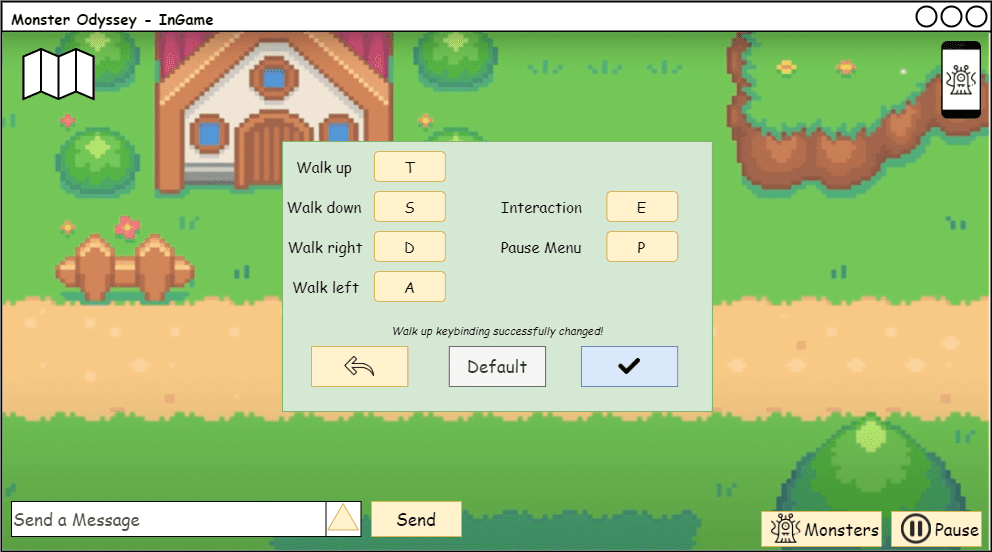
\includegraphics[width=\textwidth]{images/mockups/Bonusfeatures/Keybindings/KeybindingsSettingsChanged.png}
        \caption{Mockup: Tastenkürzel geändert}
        \label{fig: Tastenkürzel geändert}
    \end{subfigure}
    \caption{Mockup: Ändern eines Tastenkürzels}
    \label{fig: Ändern eines Tastenkürzels}
\end{figure}
\subsection{Vergleich zwischen Mockups und Implementierung}\label{subsec:vergleich-zwischen-mockups-und-implementierung-keybindings-settings}
In der Abbildung~\ref{fig: Vergleich: Einstellungen der Tastenkürzel} sind zwei Unterschiede zwischen dem Mockup und der Implementierung anzudeuten: Der Hinweis für das Ändern der Tastenkürzel wird in der Implementierung wie in der Abbildung~\ref{fig: Implementierung: Einstellungen der Tastenkürzel} nicht kursiv geschrieben, was dennoch keinen Einfluss auf die Logik der Einstellungen hat. Zudem ändert sich nach Rücksprache mit dem Kunden der Standardknopf für das Pausieren des Spiels auf die Taste „ESC“.
\begin{figure}[H]
    \centering
    \begin{subfigure}[b]{0.4\textwidth}
        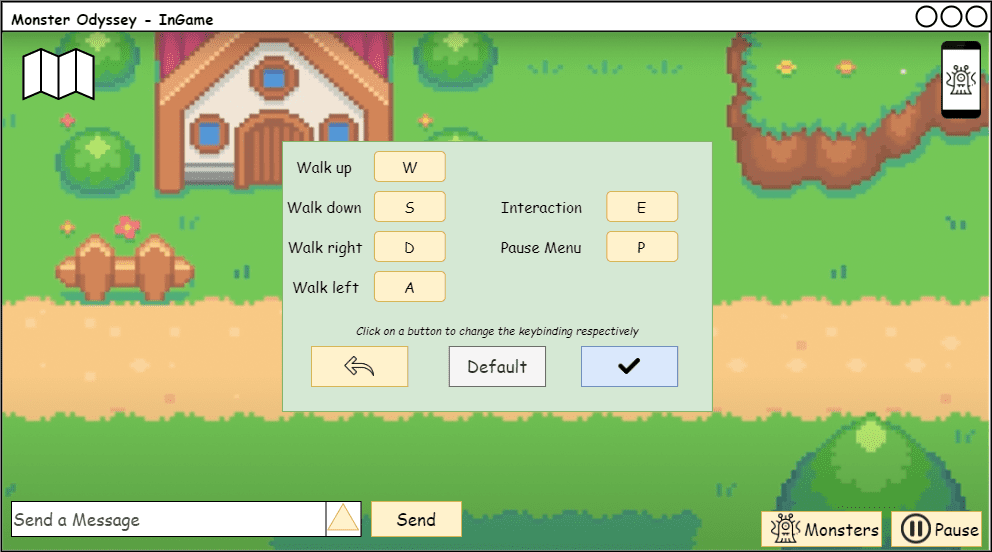
\includegraphics[width=\textwidth]{images/mockups/Bonusfeatures/Keybindings/KeybindingsSettings.png}
        \caption{Mockup: Einstellungen der Tastenkürzel}
        \label{fig: Mockup: Einstellungen der Tastenkürzel}
    \end{subfigure}
    \hfill
    \begin{subfigure}[b]{0.4\textwidth}
        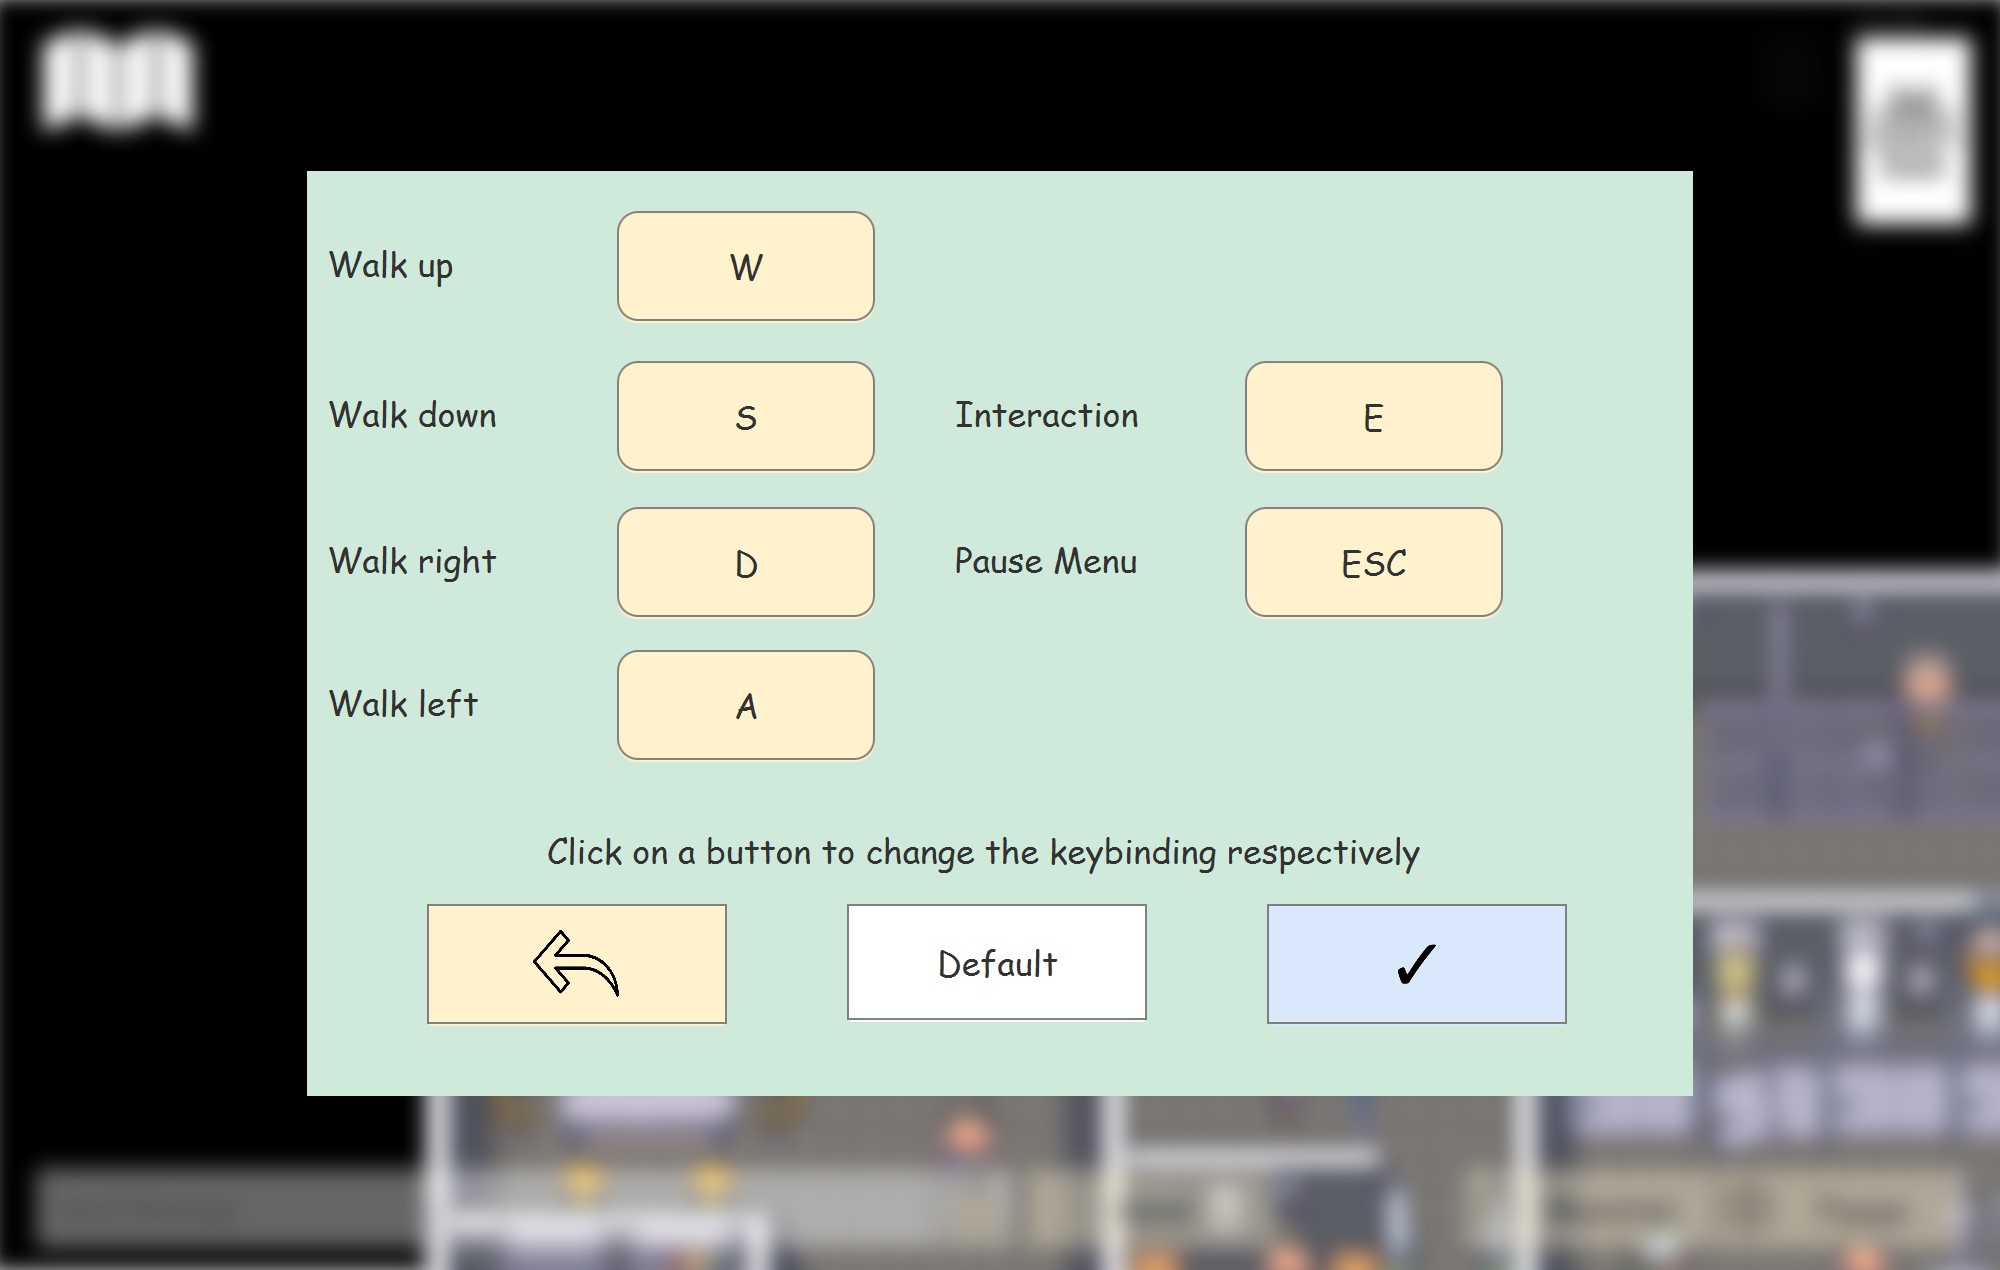
\includegraphics[width=\textwidth]{images/implementation/Bonusfeatures/Keybindings/SettingsKeyImp.png}
        \caption{Implementierung: Einstellungen der Tastenkürzel}
        \label{fig: Implementierung: Einstellungen der Tastenkürzel}
    \end{subfigure}
    \caption{Vergleich: Einstellungen der Tastenkürzel}
    \label{fig: Vergleich: Einstellungen der Tastenkürzel}
\end{figure}
Des Weiteren besteht in der Abbildung~\ref{fig: Vergleich: Warten auf Eingabe} ein wesentlicher Unterschied zwischen dem Mockup und der Implementierung. Beim Drücken einer Taste werden die anderen Tasten in der Implementierung wie in der Abbildung~\ref{fig: Implementierung: Warten auf Eingabe} kurzzeitig deaktiviert, damit der Nutzer keine andere Taste gleichzeitig ändern kann. Außerdem wird der Hinweistext im Fenster nicht zentriert, was dennoch keine Funktionalitätsänderung mit sich führt.
\begin{figure}[H]
    \centering
    \begin{subfigure}[b]{0.4\textwidth}
        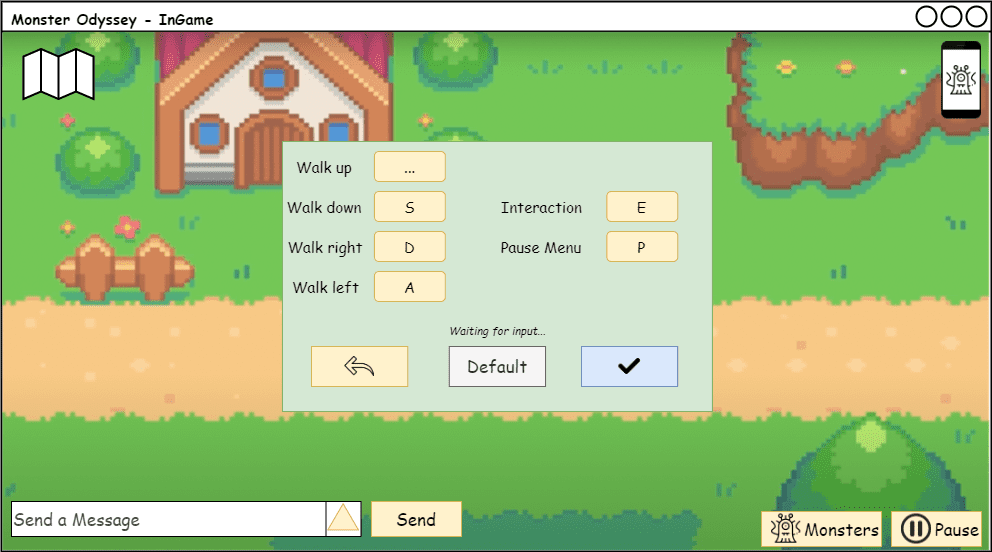
\includegraphics[width=\textwidth]{images/mockups/Bonusfeatures/Keybindings/KeybindingsSettingsWaitingForInput.png}
        \caption{Mockup: \phantom{aaaaaaa} Warten auf Eingabe}
        \label{fig: Mockup: Warten auf Eingabe}
    \end{subfigure}
    \hfill
    \begin{subfigure}[b]{0.4\textwidth}
        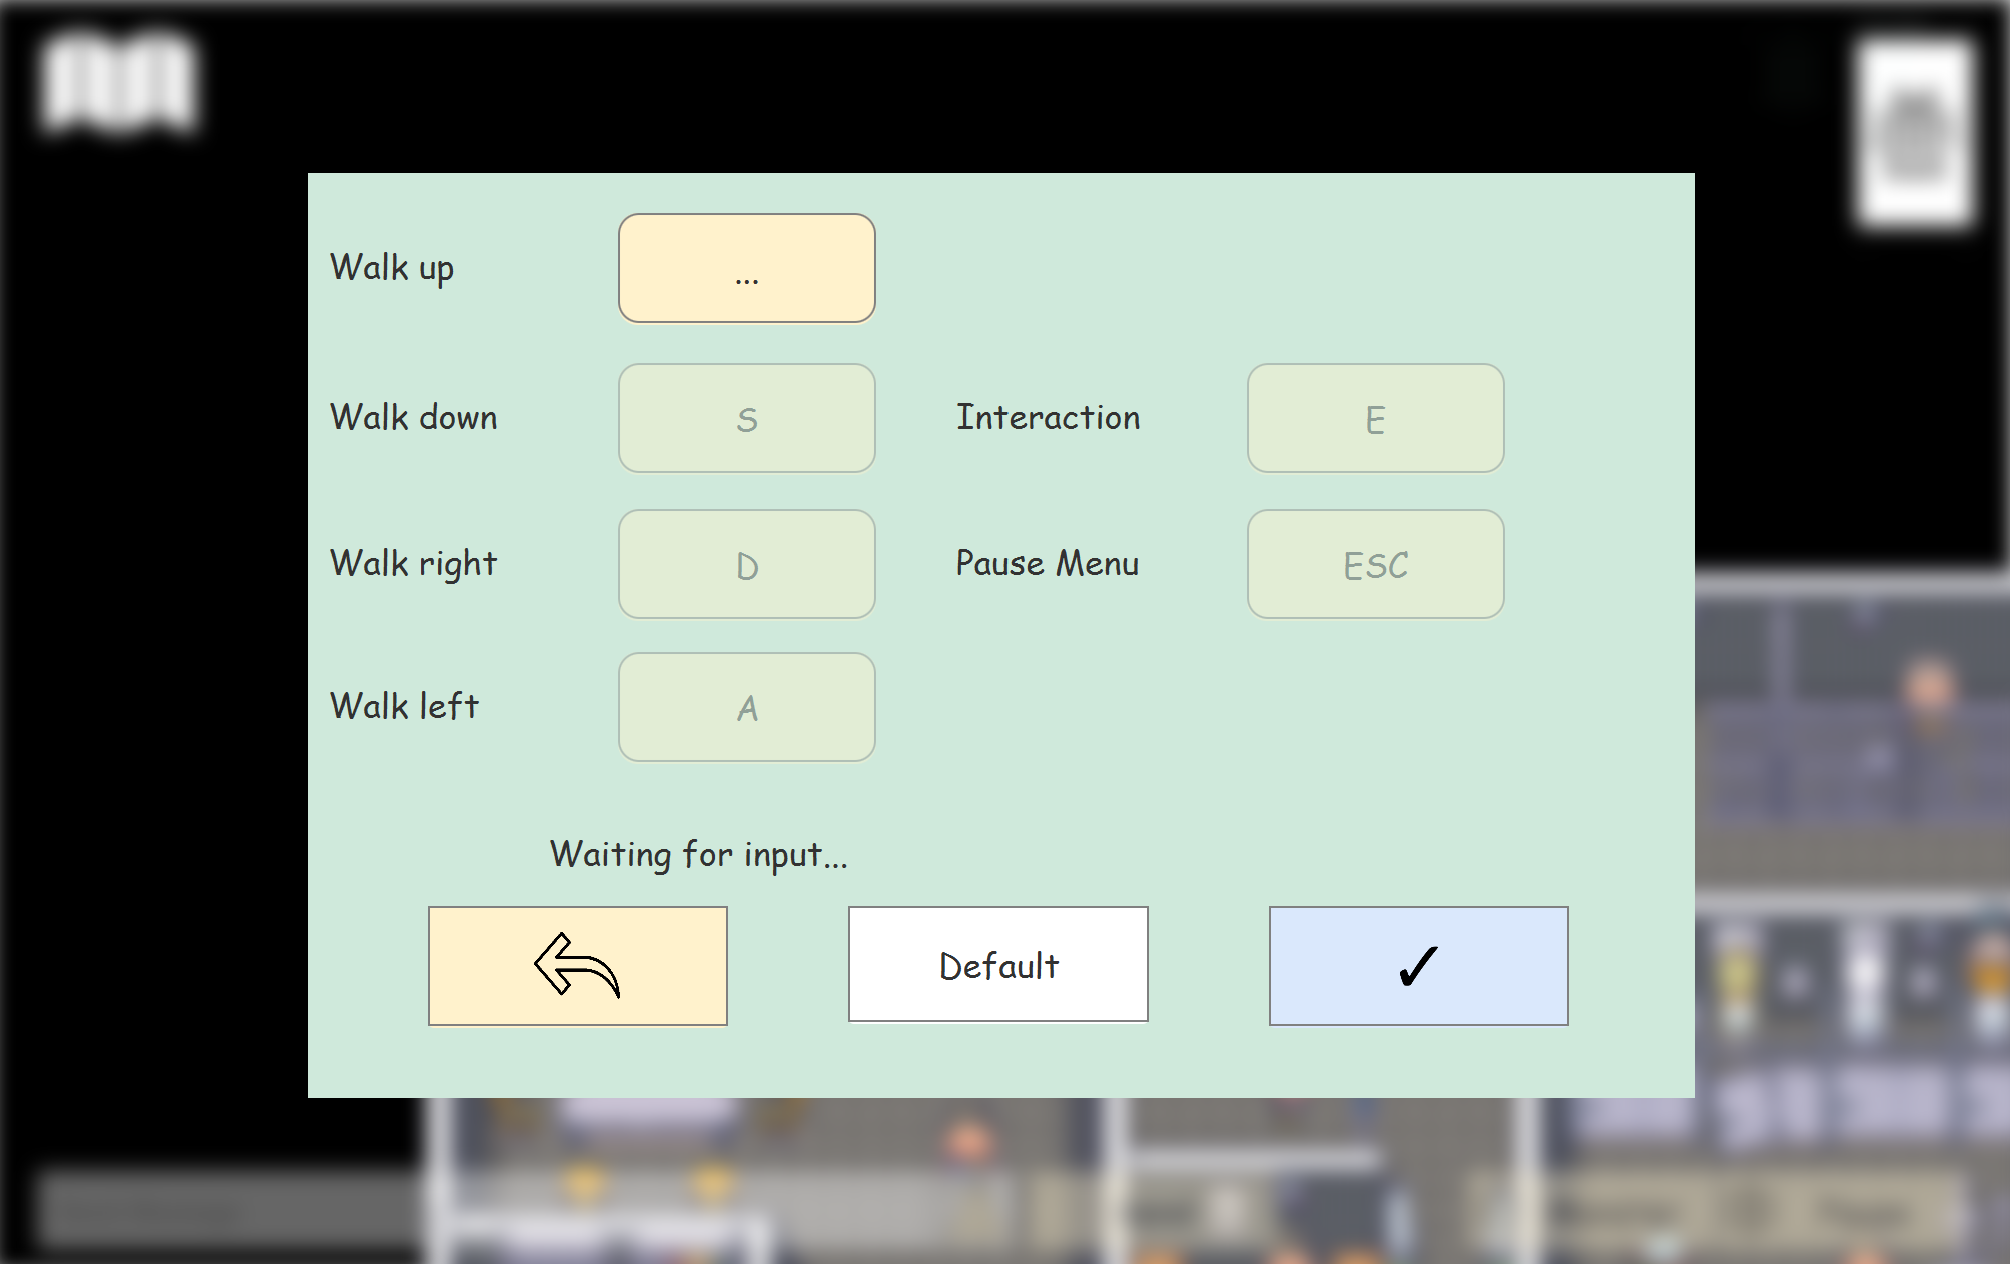
\includegraphics[width=\textwidth]{images/implementation/Bonusfeatures/Keybindings/WaitForInput.png}
        \caption{Implementierung: Warten auf Eingabe}
        \label{fig: Implementierung: Warten auf Eingabe}
    \end{subfigure}
    \caption{Vergleich: Warten auf Eingabe}
    \label{fig: Vergleich: Warten auf Eingabe}
\end{figure}
Zuletzt ist in der Abbildung~\ref{fig: Vergleich: Eingabe erfolgt} ein weiterer wichtiger Unterschied zu sehen: Die Tastenänderung erfolgt vom Nutzer in der Implementierung wie in der Abbildung~\ref{fig: Implementierung: Eingabe erfolgt} nur dann, wenn der Nutzer den Bestätigungsknopf gedrückt hat. Somit kann der Nutzer selbst entscheiden, ob er seine Änderungen rückgängig machen möchte, die er getätigt hatte.
\begin{figure}[H]
    \centering
    \begin{subfigure}[b]{0.4\textwidth}
        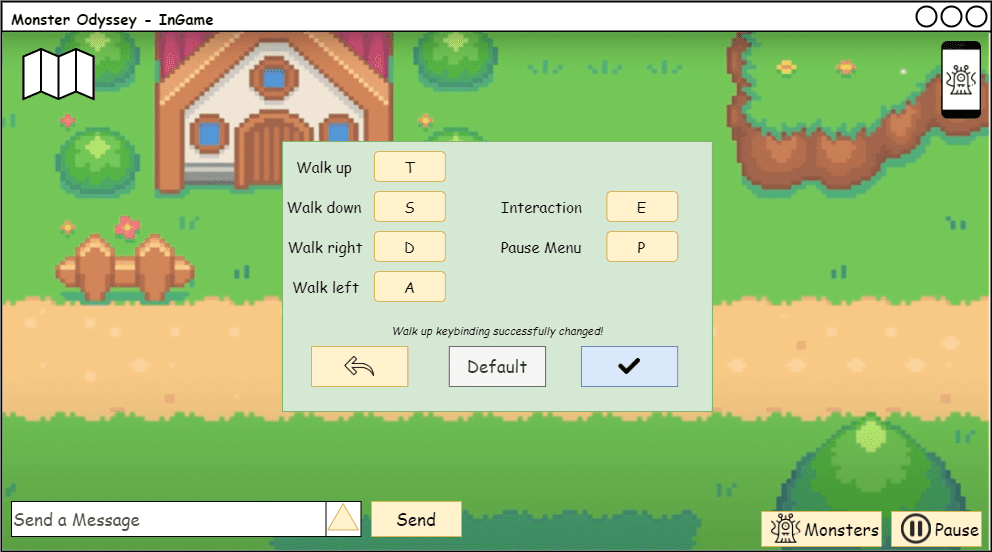
\includegraphics[width=\textwidth]{images/mockups/Bonusfeatures/Keybindings/KeybindingsSettingsChanged.png}
        \caption{Mockup: \phantom{aaaaaaa} Eingabe erfolgt}
        \label{fig: Mockup: Eingabe erfolgt}
    \end{subfigure}
    \hfill
    \begin{subfigure}[b]{0.4\textwidth}
        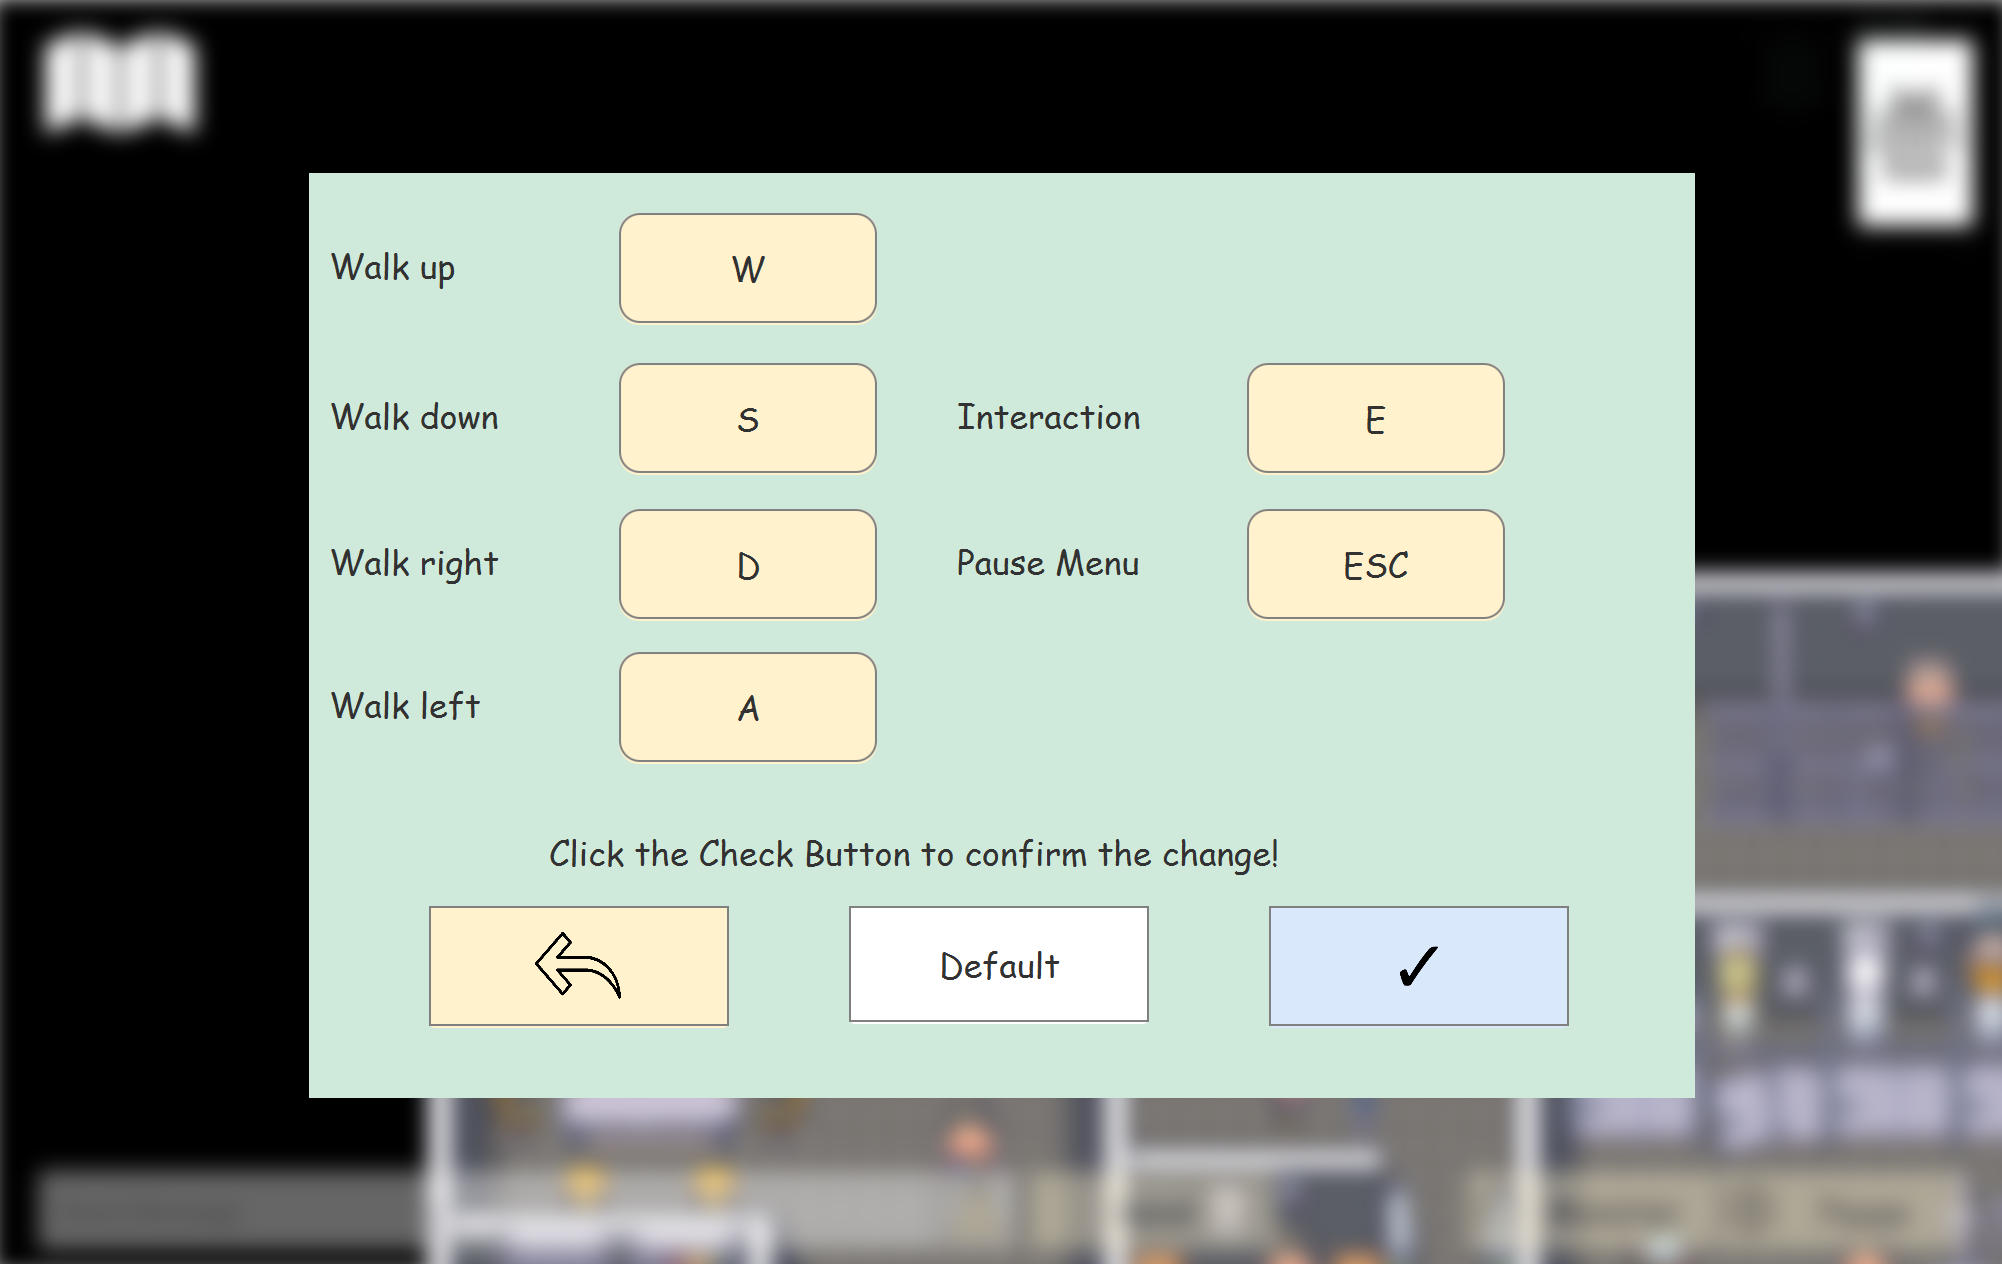
\includegraphics[width=\textwidth]{images/implementation/Bonusfeatures/Keybindings/InputErfolgt.png}
        \caption{Implementierung: Eingabe erfolgt}
        \label{fig: Implementierung: Eingabe erfolgt}
    \end{subfigure}
    \caption{Vergleich: Eingabe erfolgt}
    \label{fig: Vergleich: Eingabe erfolgt}
\end{figure}
